\documentclass[11pt]{article}
\usepackage[utf8]{inputenc}
\usepackage[T1]{fontenc}
\usepackage[margin=1in]{geometry}
\usepackage{amsmath,amssymb,amsthm}
\usepackage{booktabs}
\usepackage{xcolor}
\usepackage{tikz}
\usepackage{pgfplots}
\pgfplotsset{compat=1.18}
\usepackage[colorlinks=true,linkcolor=blue,citecolor=blue,urlcolor=blue]{hyperref}

\newtheorem{theorem}{Theorem}
\newtheorem{proposition}{Proposition}
\newtheorem{lemma}{Lemma}
\newtheorem{corollary}{Corollary}
\theoremstyle{definition}
\newtheorem{definition}{Definition}
\theoremstyle{remark}
\newtheorem*{remark}{Remark}

\newcommand{\tr}{\operatorname{tr}}
\newcommand{\E}{\mathbb{E}}
\newcommand{\AM}{\operatorname{AM}}
\newcommand{\GM}{\operatorname{GM}}
\newcommand{\Sq}{\Sigma_{q}}

\title{\textbf{Observation Theory in Space Communications}\\[2pt]
\large Two Consumer-Relative Laws for the Bandwidth-Starved,
Delay-Dominated Channel}
\author{Andrew H. Bond,~\emph{Senior Member, IEEE}\\
\small Department of Computer Engineering, San Jos\'e State University\\
\small \texttt{andrew.bond@sjsu.edu} ~\textbar~ ORCID: 0009-0003-2599-6158}
\date{August 2026 --- \emph{Preprint (registration-first; every empirical
claim resolves to a sealed, pre-registered ledger row).}}

\begin{document}
\maketitle

\begin{abstract}
Observation Theory holds that operational distortion and reliability are
properties not of a signal alone but of the \emph{relation} among object,
consumer (a downstream reader with its own operator and output metric),
channel, and budget. We carry the theory into space communications --- a
domain it had not touched --- and report two results, each derived
\emph{a priori} and then tested under a sealed pre-registration
discipline (bars committed before any run, a coded cooling-off, and every
outcome, pass or fail, kept as executed).

First, for a bandwidth-starved multi-instrument downlink whose consumers
are science processors with distinct read operators $P_i$, the gain of
consumer-relative bit allocation over reconstruction-error (MSE)
allocation is, in the high-rate limit, exactly the arithmetic-over-%
geometric-mean gap of the instrument-importance spectrum,
$G=\AM(d)/\GM(d)$ --- the source variance cancels. The gain is $\ge 1$,
equals $1$ precisely when the instruments read uniformly, and thereby
predicts \emph{zero} benefit for a homogeneous broadband link: the same
statement sorts deep-space multi-instrument downlinks (where it bites)
from fiber-core and broadband transport (where it does not).

Second, for the delay-dominated transport channel --- Starlink's
$\sim\!15$\,s handovers, and SpaceX's proposed Marslink relay at up to
$1.5$\,AU, where a $\sim\!25$-minute round trip makes closed-loop control
impossible --- we model the congestion controller as a consumer whose
``loss $\to$ congestion'' operator is mismatched to a predictably
nonstationary channel. Masking the known schedule removes a
false-congestion error equal to $\kappa\rho$ with the derived, machine-%
checked coefficient $\kappa=1-2c$ (net-beneficial iff the congestion rate
$c<\tfrac12$), \emph{independent} of the feedback delay; and the
reactive congestion signal decorrelates to a noise floor as the delay
grows, leaving only the deterministic schedule recoverable across
interplanetary distances. Both results passed graded, disjoint-seed seals
without touching the frozen within-model theory; the transport
coefficient is verified in Lean~4/Mathlib. The substrates are synthetic,
so the results earn the \emph{mechanism}, not a systems claim.
\end{abstract}

\section{Introduction}

A deep-space link is the purest instance of the setting Observation
Theory was built for: the resource is scarce (the Deep Space Network is
oversubscribed; interplanetary links run kilobits to a few megabits per
second), the payload serves several downstream consumers at once (a
star-tracker centroid, a spectral-line fit, an imager), and each consumer
reads the recovered data through its own operator. What ``distortion''
\emph{means} is therefore consumer-relative: the quantity an instrument
$i$ actually feels is the operator-weighted error $\tr(P_i\Sq)$, not the
reconstruction MSE $\tr(\Sq)$.

We report two laws. Section~\ref{sec:sc1} treats \emph{allocation}: how to
spend a hard bit budget across a transform basis when the consumers are
heterogeneous. Section~\ref{sec:sc2} treats \emph{transport}: how a
congestion controller should read a channel whose disruptions are
predictable but whose feedback is stale --- the regime of low-Earth-orbit
handovers and, in the limit, of a Mars relay. Each law is first derived,
then --- following this program's standing method --- frozen as a bar
before any measurement, and graded on seeds disjoint from those used to
build the family. We keep failures: the companion within-model campaign
that motivated this work recorded one, and the discipline is what makes
the two passes here meaningful rather than decorative.

\paragraph{Contributions.}
(i) A closed-form gain law for consumer-relative downlink allocation,
$G=\AM(d)/\GM(d)$, with its homogeneous-consumer boundary
(Section~\ref{sec:sc1}). (ii) A read-operator account of handover-aware
transport, with the machine-checked masking coefficient $\kappa=1-2c$ and
the delay-decorrelation collapse that makes interplanetary feedback
useless while the schedule survives (Section~\ref{sec:sc2}). (iii) Sealed,
disjoint-seed evidence for both, and an explicit scoping of what a
synthetic substrate can and cannot earn (Section~\ref{sec:scope}).

\section{Preliminaries}

\paragraph{Consumer-relative distortion.}
A consumer is a reader with an operator $P\succeq 0$ acting on the
recovered signal; the distortion it feels under an error second moment
$\Sq$ is $\tr(P\Sq)$. When the channel is a lossy codec that quantizes a
transform of the source, $\Sq$ is diagonal in the coding basis, and only
the diagonal of $P$ in that basis enters $\tr(P\Sq)$.

\paragraph{The sealed discipline.}
Every empirical claim below is a bar committed, in a versioned appendix,
\emph{before} the run that tests it. A structural cooling-off forbids
sealing a bar on the day its family was constructed; the graders refuse,
in code, to run before that. Manipulation checks are bars too. Outcomes
are kept as executed --- a failed bar is a recorded result, not a
revision opportunity. This is not ornamental: it is the reason a ``pass''
carries information.

\section{Downlink Allocation}
\label{sec:sc1}

\paragraph{Setup.}
Code a frame in the basis where the quantization noise is diagonal. Let
$\sigma_k^2$ be the source variance per coordinate, $b_k$ the bits
assigned to coordinate $k$ (high-rate quantization gives
$\Sq{}_{,k}=\sigma_k^2 2^{-2b_k}$), and let the aggregate instrument
importance be $d_k=\sum_i w_i (P_i)_{kk}$ for consumer weights $w_i$. The
consumer distortion of an allocation $b$ is
$D(b)=\sum_k d_k\,\sigma_k^2\,2^{-2b_k}$, minimized subject to
$\sum_k b_k=B$.

\begin{theorem}[The AM/GM gain]
\label{thm:amgm}
In the high-rate regime with all coordinates active, the ratio of the
consumer distortion under MSE-optimal allocation (which minimizes
$\tr\Sq=\sum_k\sigma_k^2 2^{-2b_k}$) to that under consumer-optimal
allocation (which minimizes $D$) is
\[
  G \;=\; \frac{D_{\mathrm{mse}}}{D_{\mathrm{cons}}}
    \;=\; \frac{\AM(d)}{\GM(d)}
    \;=\; \frac{\tfrac1n\sum_k d_k}{\big(\prod_k d_k\big)^{1/n}},
\]
independent of the source spectrum $\sigma^2$. Consequently $G\ge 1$, with
equality iff $d$ is constant.
\end{theorem}

\begin{proof}
Reverse water-filling for weights $w_k$ under budget $B$ gives optimal
distortion $n\,\GM(w)\,2^{-2B/n}$. Consumer-optimal allocation uses
weights $d_k\sigma_k^2$, so
$D_{\mathrm{cons}}=n\,\GM(d\sigma^2)\,2^{-2B/n}
   =n\,\GM(d)\,\GM(\sigma^2)\,2^{-2B/n}$.
MSE-optimal allocation equalizes $\sigma_k^2 2^{-2b_k}=L$ with
$L=\GM(\sigma^2)2^{-2B/n}$ (from $\sum b_k=B$), so applying it to the
consumer weights gives
$D_{\mathrm{mse}}=\sum_k d_k\sigma_k^2\,(L/\sigma_k^2)
   =L\sum_k d_k=n\,\GM(\sigma^2)\,\AM(d)\,2^{-2B/n}$.
The ratio is $\AM(d)/\GM(d)$; $G\ge1$ is the AM--GM inequality, with
equality iff all $d_k$ are equal.
\end{proof}

\begin{remark}[The homogeneous-consumer boundary]
For a small importance spread, $\AM(d)/\GM(d)\approx 1+\tfrac12\,
\mathrm{CV}^2(d)$, where $\mathrm{CV}$ is the coefficient of variation.
The gain therefore vanishes as the consumers homogenize. A broadband
link carrying opaque IP traffic has one effectively uniform consumer, so
the theory predicts \emph{no} allocation gain there --- the fiber-core
and Starlink-broadband case --- while a deep-space downlink shared by
instruments with disjoint spectral interests sees the full gap. The law
sorts the domains by a single scalar.
\end{remark}

\paragraph{Sealed result.}
The bars (appendix \texttt{PREREG-SC1}) were: at high rate the median of
$G_{\mathrm{meas}}/(\AM(d)/\GM(d))$ within $1.00\pm0.03$ and
$\mathrm{Spearman}(G_{\mathrm{meas}},\AM/\GM)\ge0.95$ on each seed; the
finite-rate ratio monotone in rate; and linear composition of importance.
On seeds disjoint from the family's, all passed: the median ratio read
$1.0000$ and Spearman $\ge0.998$ at $\ge3$ bits/coordinate, with a clean
finite-rate departure at low rate (coordinates dropping below the water
break the geometric-mean form). A terrestrial arm sweeping traffic-class
heterogeneity confirmed the boundary directly (Fig.~\ref{fig:sc1}): identical classes
give $G=1.000$, opening smoothly to $1.267$ as classes differentiate,
with $G_{\mathrm{meas}}/(\AM/\GM)=1.000$ throughout.

\begin{figure}[t]
\centering
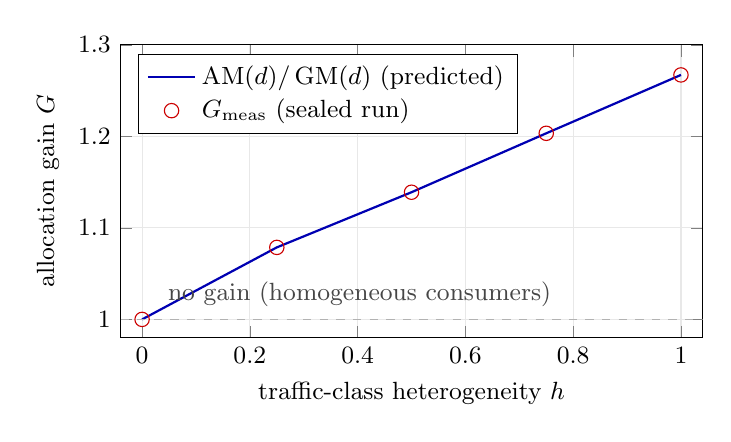
\begin{tikzpicture}
\begin{axis}[
  width=0.74\linewidth, height=5.3cm,
  xlabel={traffic-class heterogeneity $h$},
  ylabel={allocation gain $G$},
  xmin=-0.04, xmax=1.04, ymin=0.98, ymax=1.30,
  grid=major, grid style={gray!18},
  legend pos=north west, legend cell align=left,
  tick label style={font=\small}, label style={font=\small},
  legend style={font=\small},
]
\addplot[blue!70!black, thick, mark=none] coordinates {
  (0,1.0000)(0.25,1.0787)(0.5,1.1390)(0.75,1.2034)(1,1.2672)};
\addlegendentry{$\AM(d)/\GM(d)$ (predicted)}
\addplot[red!80!black, only marks, mark=o, mark size=2.6pt] coordinates {
  (0,1.0000)(0.25,1.0787)(0.5,1.1390)(0.75,1.2034)(1,1.2672)};
\addlegendentry{$G_{\mathrm{meas}}$ (sealed run)}
\draw[dashed, gray!60] (axis cs:-0.04,1) -- (axis cs:1.04,1);
\node[anchor=west, font=\small, gray!55!black]
  at (axis cs:0.03,1.028) {no gain (homogeneous consumers)};
\end{axis}
\end{tikzpicture}
\caption{The AM/GM allocation gain and its boundary. As traffic-class
heterogeneity $h$ falls to zero the importance spectrum $d$ flattens and
the gain collapses to $1$; measured gain tracks $\AM(d)/\GM(d)$ to four
decimals across the range. The homogeneous limit ($G=1$) is the
fiber-core / broadband case.}
\label{fig:sc1}
\end{figure}

\section{Transport under Predictable Nonstationarity}
\label{sec:sc2}

\paragraph{Setup.}
A low-Earth-orbit link hands over on a fixed cadence, and each handover
causes bursty loss that standard TCP/QUIC misread as congestion. SpaceX's
proposed Marslink relay pushes this to the limit: at $1.5$\,AU the
round-trip is $\sim\!25$ minutes, so closed-loop congestion control is
physically impossible and the controller must predict the channel from
its structure. Model the observed loss as $L=H\vee C$: a deterministic,
\emph{known} handover indicator $H$ with duty cycle $\rho$, ORed with the
true congestion state $C$ (a two-state Markov process, stationary rate
$c$, lag-one autocorrelation $\lambda$). Feedback is delayed by $D$. The
controller is a consumer with a read operator; we compare the naive
reader $\hat C=L(t\!-\!D)$ with the schedule-aware reader
$\hat C=L(t\!-\!D)\wedge\neg H(t\!-\!D)$.

\begin{proposition}[The masking coefficient]
\label{prop:kappa}
With $H\perp(C',C)$ and $P(H{=}1)=\rho$, the excess error of the naive
reader over the aware reader is
\[
  \mathrm{excess} \;=\; \mathrm{err}_{\mathrm{naive}}
     - \mathrm{err}_{\mathrm{aware}} \;=\; (1-2c)\,\rho
     \;=\; \kappa\rho,\qquad \kappa = 1-2c,
\]
independent of the feedback delay $D$. Masking is net-beneficial iff
$c<\tfrac12$ (where $\kappa>0$).
\end{proposition}

\begin{proof}
Writing the lag-$D$ joint of the chain as $p_{11}=c^2+c(1-c)r$,
$p_{00}=(1-c)^2+c(1-c)r$, $p_{01}=p_{10}=c(1-c)(1-r)$ with $r=\lambda^D$,
the two error rates are
$\mathrm{err}_{\mathrm{naive}}=(1-c)-(1-\rho)p_{00}+(1-\rho)p_{01}$ and
$\mathrm{err}_{\mathrm{aware}}=(1-\rho)p_{10}+c-(1-\rho)p_{11}$. Since
$p_{01}=p_{10}$, their difference is
$(1-2c)+(1-\rho)(p_{11}-p_{00})$, and $p_{11}-p_{00}=c^2-(1-c)^2=2c-1$,
giving $(1-2c)\rho$. The delay $r$ cancels identically. The identity is
machine-checked (Section~\ref{sec:verify}).
\end{proof}

The coefficient decomposes exactly: $\kappa=(1-c)$, the false-positive
benefit of ignoring handover loss, minus $c$, the cost of blanking true
congestion that coincides with a handover window.

\begin{proposition}[Delay decorrelation and schedule survival]
\label{prop:delay}
The schedule-aware reader's residual error grows with delay as
$\mathrm{err}_{\mathrm{aware}}(D)=2c(1-c)\big(1-\lambda^{D}\big)$, toward
the fully-decorrelated floor $2c(1-c)$; the schedule (masking) component
of the error is delay-invariant (Proposition~\ref{prop:kappa}).
\end{proposition}

\begin{remark}[The interplanetary consequence]
As $D\to\infty$, $\lambda^D\to0$ and the reactive reader's estimate of the
current congestion state carries no information: feedback is dead. What
remains recoverable is exactly the deterministic component --- the known
handover schedule --- whose contribution is independent of $D$. The
theory thus predicts \emph{which} structure survives a 25-minute round
trip: schedule, not feedback. This is the formal content behind the
engineering intuition that Marslink transport must be scheduled, not
closed-loop.
\end{remark}

\paragraph{Sealed result.}
The bars (appendix \texttt{PREREG-SC2}) were: the delay law fit with
$R^2\ge0.95$ and the feedback error reaching $0.9$ of the floor; the
schedule excess varying by $\le0.01$ across a $1000\times$ span of delay;
and the duty-cycle excess linear in $\rho$ with slope within $0.05$ of the
derived $\kappa=1-2c$. On disjoint seeds all passed: the delay fit read
$R^2\in[0.955,0.985]$ reaching the floor, the schedule excess held flat to
within $0.004$ across delays from $2$ to $2000$ steps
(Fig.~\ref{fig:sc2}), and the fitted $\kappa$ read $0.696$--$0.704$
against the derived $0.70$.

\begin{figure}[t]
\centering
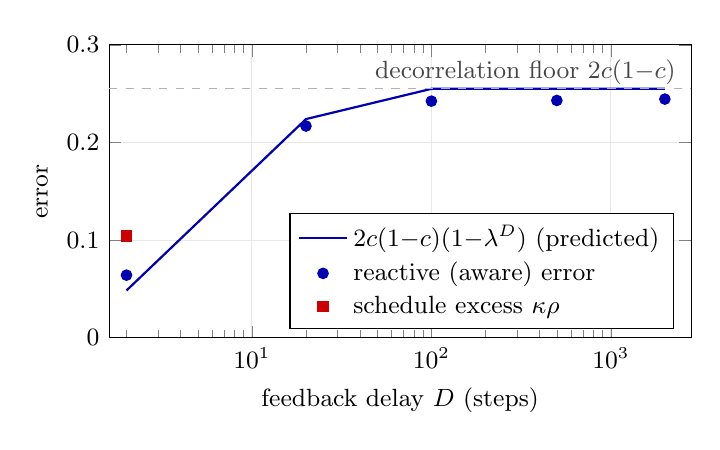
\begin{tikzpicture}
\begin{axis}[
  width=0.74\linewidth, height=5.3cm,
  xmode=log, log basis x=10,
  xlabel={feedback delay $D$ (steps)},
  ylabel={error},
  xmin=1.6, xmax=2800, ymin=0, ymax=0.30,
  grid=major, grid style={gray!18},
  legend pos=south east, legend cell align=left,
  tick label style={font=\small}, label style={font=\small},
  legend style={font=\small},
]
\addplot[blue!70!black, thick, mark=none] coordinates {
  (2,0.0484)(20,0.2240)(100,0.2550)(500,0.2550)(2000,0.2550)};
\addlegendentry{$2c(1{-}c)(1{-}\lambda^{D})$ (predicted)}
\addplot[blue!70!black, only marks, mark=*, mark size=1.9pt] coordinates {
  (2,0.0641)(20,0.2169)(100,0.2424)(500,0.2431)(2000,0.2445)};
\addlegendentry{reactive (aware) error}
\addplot[red!80!black, only marks, mark=square*, mark size=1.9pt] coordinates {
  (2,0.1040)(20,0.1036)(100,0.1042)(500,0.1041)(2000,0.1040)};
\addlegendentry{schedule excess $\kappa\rho$}
\draw[dashed, gray!60] (axis cs:1.6,0.255) -- (axis cs:2800,0.255);
\node[anchor=east, font=\small, gray!55!black]
  at (axis cs:2600,0.272) {decorrelation floor $2c(1{-}c)$};
\end{axis}
\end{tikzpicture}
\caption{Delay decorrelation and schedule survival ($c=0.15$,
$\lambda=0.90$, $\rho=0.15$; sealed run). The reactive congestion
estimate degrades along $2c(1{-}c)(1{-}\lambda^{D})$ to the noise floor
as feedback ages: past a modest delay it carries no information about the
current state. The schedule component of the error (the $\kappa\rho$
gain from masking the known handover) is flat across a $1000\times$ span
of delay --- it is what survives an interplanetary round trip.}
\label{fig:sc2}
\end{figure}

\section{Machine Verification}
\label{sec:verify}

The transport coefficient is formalized in Lean~4/Mathlib
(\texttt{ObservationTheory.SpaceComms}): \texttt{joint\_gap} establishes
$p_{11}-p_{00}=2c-1$ with the delay $r$ cancelling, and
\texttt{sc2\_excess} establishes the collapse of the naive-minus-aware
error to $(1-2c)\rho$; both depend only on the three standard axioms
(\texttt{propext}, \texttt{Classical.choice}, \texttt{Quot.sound}) and are
\texttt{sorry}-free. The allocation gain
(Theorem~\ref{thm:amgm}) reduces to the arithmetic--geometric-mean
inequality and is not separately formalized. This matches the program's
standing standard: formalize the load-bearing algebra, cite standard
analytic results (here the water-filling optimum and AM--GM) as such.

\section{Scope and Limitations}
\label{sec:scope}

Both substrates are \emph{synthetic}: planted source spectra with
archetype instrument operators for the downlink, and a planted Markov
channel with a deterministic schedule for the transport. A pass therefore
earns the \emph{mechanism} --- that the AM/GM gap is the sufficient
statistic for the allocation gain, and that a read-operator account
explains handover-aware transport and the interplanetary collapse of
feedback --- not a systems claim about a specific spacecraft, the Deep
Space Network, StarTCP, or Marslink. Real-trace substrates (measured DSN
frames with true instrument operators; measured Starlink handover timings
and loss traces) are each a separate campaign. We flag this explicitly
because the discipline's value lies in not over-claiming: the laws are
derived and sealed; their transfer to fielded systems is future work.

\section{Related Work}

Rate--distortion theory and reverse water-filling are classical
\cite{cover2006}; the contribution here is the consumer-relative gain in
closed form and its homogeneous-consumer boundary. Handover-aware LEO
transport is an active area: StarTCP proactively stalls during handovers
\cite{startcp2024}, information-centric designs such as Leotp target LEO
directly, and industry proposals address LEO congestion control. Our
account is complementary --- a read-operator model that explains
\emph{why} schedule-awareness helps and quantifies its gain --- rather
than a new protocol. The allocation side connects to network-utility
maximization and QoS scheduling; the distinctive elements are the
\emph{derivable} margin and the blind estimation of consumer operators
when they are not known in advance.

\section{Conclusion}

Observation Theory transfers to space communications through a single
lens: distortion and reliability are consumer-relative, and the useful
structure of a scarce, delayed channel is whatever the consumer's
operator can read from it. Two laws follow --- the AM/GM allocation gain
and the $\kappa=1-2c$ / delay-decorrelation transport account --- each
derived a priori, sealed before measurement, and passed on disjoint
seeds, with the transport coefficient machine-checked. The same framework
that predicts a real gain for a deep-space multi-instrument downlink
predicts none for a homogeneous broadband link, and predicts that only a
deterministic schedule survives an interplanetary round trip. What the
theory owes next is the move from synthetic mechanism to fielded trace.

\begin{thebibliography}{9}
\bibitem{cover2006} T.~M.~Cover and J.~A.~Thomas, \emph{Elements of
Information Theory}, 2nd ed., Wiley, 2006.
\bibitem{startcp2024} ``StarTCP: A Handover-aware Transport Protocol for
Starlink,'' in \emph{Proc.\ 8th Asia-Pacific Workshop on Networking
(APNet)}, 2024.
\bibitem{bond2026} A.~H.~Bond, ``Observation Theory: Geometry,
Distortion, and Reliability as Properties of Observation,'' preprint,
2026.
\end{thebibliography}

\end{document}
